\chapter{Second-Order Blind Identification}
\label{ch:sobi}

Second-Order Blind Identification (SOBI) is a Blind Source Separation technique that separates observed mixtures by exploiting differences in the temporal structure of the sources. Unlike ICA, which relies mainly on non-Gaussianity, SOBI is limited to second-order statistics like time-lagged covariance matrices \cite{pan_review_2022}.

This chapter presents the basic foundations, assumptions and implementation of the SOBI algorithm, followed by its evaluation in the proposed weak-source separation problem.


\section{Assumptions}
\label{sec:sobi_assumptions}
As the ICA algorithm, SOBI relies on a series of assumptions that should be at least partially satisfied for the separation to be effective. Some of these assumptions are common to both methods, such as the presence of a linear instantaneous mixture (or small delays), a full-rank mixing matrix $A$ and a number of observations greater than or equal to the number of sources, as discussed in Section \ref{sec:ica_assumptions}. Therefore, this section focuses on the assumptions that are specific to SOBI and explain their relevance in the context of the proposed problem.



\begin{itemize}

    \item \textbf{Sources have temporal structures} 
    \[ 
        \mathbf{\quad R_s(\tau)\neq0}
    \]
    SOBI requires that samples close in time should have some relationship with each other. For EMG, this is reasonable since muscle activations have temporal continuity and their RMS envelope changes progressively over time.
    \item \textbf{Sources have different temporal structures}
    \[
        \mathbf{ R_{s1}(\tau)\not\approx R_{s2}(\tau)}
     \]
    This assumption is essential because SOBI separates sources through differences in their temporal patterns. If two sources evolve similarly over time, reliable separation becomes difficult, which may occur for nearby or functionally related EMG sources.
    \item \textbf{Sources have no time-lagged cross-correlation}
    \[
    \mathbf{E\left[s_i(t)s_j(t-\tau)\right] = 0, \quad \forall \quad i\neq j}
    \]
    This means that each source may be correlated with itself over time, but not with lagged versions of other sources. In EMG, this assumption can be challenged when several muscles are activated simultaneously.
\end{itemize}

  

\section{Working principle}

Second-Order Blind Identification starts from the same linear mixture model introduced previously and shares initial preprocessing steps with ICA. The observed mixtures are first centered to remove their mean and then whitened so that the channels become uncorrelated and have unit variance. After whitening, the separation problem is reduced to finding an orthogonal transformation that removes the remaining mixing effect in $\mathbf{z}(t)$. Instead of searching for the rotation that maximizes non-Gaussianity, as in ICA, SOBI estimates this transformation using delayed covariance matrices. For a given delay $\tau$, Equation \ref{eq:covariance_matrix_sobi} defines the covariance matrix of the whitened observations $\mathbf{z}(t)$.

\begin{equation}
    \mathbf{R}_z(\tau) = E\left[\mathbf{z}(t)\mathbf{z}^T(t-\tau)\right]\label{eq:covariance_matrix_sobi}
\end{equation}

Given the assumptions presented in the previous section (\ref{sec:sobi_assumptions}), the delayed covariance matrix of the sources should be diagonal, since each source may be correlated with itself over time but not with delayed versions of the other sources. This is shown in Equation \ref{eq:sobi_diagonal_covariance}.
\begin{equation}
    \mathbf{R}_s(\tau) =
\begin{bmatrix}
R_{s_1}(\tau) & \approx0 \\
\approx0 & R_{s_2}(\tau)
\end{bmatrix}
\label{eq:sobi_diagonal_covariance}
\end{equation}

This implies that each source only contributes to its own autocorrelation term. Since the whitened observations are still a rotated version of the original sources, SOBI searches for a rotation matrix $\mathbf{B}$ that makes the delayed covariance matrices of the whitened data as diagonal as possible. 

\begin{equation}
    \mathbf{B}\mathbf{R}_z(\tau)\mathbf{B}^T \approx \mathbf{D}=\begin{bmatrix}
        d_1(\tau) & 0 \\
        0 &d_2(\tau)
    \end{bmatrix}
\end{equation}
where $d_1,d_2$ are the autocorrelation values of the source signals at a given lag. Nevertheless, this condition has to be applied to several delays. SOBI considers delays $\tau_1,\tau_2,\dots,\tau_K$ as each delay contains significant temporal information about the sources. Therefore, the goal is to find a unique rotation matrix $\mathbf{B}$ that approximately diagonalizes all delayed covariance matrices at considered delays. 

\begin{equation}
    \mathbf{B}\mathbf{R}_z(\tau_k)\mathbf{B}^T \approx \mathbf{D}_k \qquad \forall k=1,2,\dots,K
\end{equation}
where $\mathbf{D}_k$ is an approximately diagonal matrix for the delay $\tau_k$. This process is called \textbf{joint diagonalization}, since this unique transformation is applied jointly to all delayed covariance matrices. Joint diagonalization can be implemented in different ways, but
it essentially evaluates a series of rotations and selects the one that minimizes the energy outside the main diagonal of these matrices. This idea is expressed in Equation \ref{eq:sobi_joint_diag}.

\begin{equation}
\mathbf{B}^{\star}
    =
    \arg\min_{\mathbf{B}}
    \sum_{k=1}^{K}
    \operatorname{off}
    \left(
    \mathbf{B}\mathbf{R}_z(\tau_k)\mathbf{B}^T
    \right), \qquad 
    \operatorname{off}(\mathbf{M})
    =
    \sum_{i \neq j} M_{ij}^{2}
    \label{eq:sobi_joint_diag}
\end{equation}

Overall, SOBI has a geometric interpretation considerably similar to the one presented for ICA in Figure \ref{fig:ica_geometry}, since both methods reduce the separation problem to a single rotation of the whitened observations. However, the principle used to select this rotation is completely different. While ICA searches the rotation that maximizes non-Gaussianity, SOBI searches for the rotation that jointly diagonalizes the time lagged covariance matrices.

\section{Implementation}
Unlike FastICA, which is available through well-established public libraries such as \texttt{scikit-learn}, \uline{SOBI does \textbf{not} have an equally standardized implementation that could be directly applied to the signals considered in this thesis}. Consequently, a custom SOBI implementation was developed, allowing greater control over the selection of time delays and the approximate joint diagonalization procedure. 

More specifically, a \textbf{Jacobi/Givens rotation strategy} was used for the joint diagonalization \cite{fevotte_pivot_nodate,van_der_veen_joint_2001}. This procedure essentially aims to find the matrix $\mathbf{B}$ by progressively combining 2D rotation matrices. For each pair $(p,q)$, the Givens rotation $G_{p,q}(\theta)$ is defined as a matrix where the only non-trivial part is the 2x2 acting rows and columns $p$ and $q$. This rotation is applied to every delayed covariance matrix $\mathbf{R}_z(\tau_k)$ at the same time the $\mathbf{B}$ matrix is updated, like shown in Equation \ref{eq:givens_update}.

\begin{equation}
    \mathbf{R}_z(\tau_k)
    \leftarrow
    \mathbf{G}_{pq}(\theta)
    \mathbf{R}_z(\tau_k)
    \mathbf{G}_{pq}^{T}(\theta), \qquad
    \mathbf{B}
    \leftarrow
    \mathbf{G}_{pq}(\theta)\mathbf{B}
    \label{eq:givens_update}
\end{equation}
For each $(p,q)$ pair, the elements of $\mathbf{R}_z(\tau_k)$ are used to compute the next rotation angle as defined in Equations \ref{eq:jacobi_a_g} and \ref{eq:jacobi_angle_computation}.

\begin{equation}
    \begin{bmatrix}
a_{pp} & a_{pq} \\
a_{pq} & a_{qq}
\end{bmatrix}, 
\qquad 
g_{11}
    =
    \sum_{k=1}^{K}
    \left(
        a_{pp}^{(k)} - a_{qq}^{(k)}
    \right), \qquad
g_{12}
    =
    \sum_{k=1}^{K}
    2a_{pq}^{(k)}
    \label{eq:jacobi_a_g}
\end{equation}

\begin{equation}
    \theta
    =
    \frac{1}{2}
    \operatorname{atan2}
    \left(
        g_{12}, g_{11}
    \right)
    \label{eq:jacobi_angle_computation}
\end{equation}
Finally, the algorithm repeats this process until either all the $(p,q)$ pairs are included or consecutive iterations do not significantly minimize off-diagonal energy. After $\mathbf{m}$ iterations ($\leq N$ dimensions), the final $\mathbf{B}$ matrix is summarized as expressed in Equation \ref{eq:jacobi_final_B}.

\begin{equation}
    \mathbf{B}
    =
    \mathbf{G}_{p_m q_m}(\theta_m)
    \cdots
    \mathbf{G}_{p_2 q_2}(\theta_2)
    \mathbf{G}_{p_1 q_1}(\theta_1)
    \label{eq:jacobi_final_B}
\end{equation}
In the experiments of this thesis, only two sources are considered so the \uline{computation is simplified to a single Givens rotation $G_{12}(\theta)$}. However, the function was implemented for a generic NxN dimension input. \textbf{See code in Appendix \ref{app:joint_diag_code} for reference}. 

\clearpage

\noindent With a joint diagonalization strategy defined, the SOBI implementation can be divided into four main sections.

\begin{itemize}
    \item \textbf{Preprocessing:} center and whiten the data (already mentioned in Chapter \ref{ch:preprocessing}). However, it is crucial to keep the whitening matrix $\mathbf{V}$ to later build the separation matrix $\mathbf{W}$.\item \textbf{Delayed covariance estimation:} compute an array of lagged covariance matrices for a list $T$ of delays. This step is explicitly included in the SOBI function.
    \item \textbf{Jointdiagonalization:} applies the Jacobi/Givens stategy detailed in this section to find the matrix $\mathbf{B}$.
    \item \textbf{Separation matrix:} combine matrix $\mathbf{B}$ with whitening transform $V$ to obtain final separation matrix $W$.
\end{itemize}

\noindent Listing \ref{lst:sobi_pseudocode} illustrates the general SOBI pseudocode followed in this thesis. \textbf{For full code implementation reference, see Appendix \ref{app:sobi_code}}

\begin{lstlisting}[
style=pseudocode,
caption={SOBI algorithm pseudocode.},
label={lst:sobi_pseudocode},
mathescape=true
]
Input: Observed EMG matrix X, number of components K,
       set of delays T, tolerance epsilon, maximum iterations Imax

Output: Estimated sources S_hat and separation matrix W

//Preprocessing
Xc <- X - mean(X)
Z, V <- Whiten(Xc, K)
//Delayed covariance estimation
R_list <- LaggedCovarianceMatrices(Z, T)

//Joint diagonalization
B <- IdentityMatrix(K)
for sweep = 1 to Imax
    B_old <- B
    B <- JacobiJointDiagonalizationStep(B, R_list)
    delta <- OffDiagonalEnergy(R_list)
    if delta < epsilon
        break
    end
end
//Source estimation
W <- B * V
S_hat <- Xc * W^T

return S_hat, W
\end{lstlisting}

\section{Experiments}

Once Second-Order Blind Identification is explained and implemented, it is crucial to test its performance with EMG signals. Since ICA already works relatively well in some experimental scenarios, this section aims to compare and ultimately assess if SOBI is better suited to separate EMG signals. Additionally, different scenarios are tested in order to understand when the two algorithms may or may not behave similarly. Finally, a conclusion about SOBI's role in EMG signal separation is included at the end of this section.

\subsection{TMR Database}

Figure \ref{fig:sobi_results_tmr} illustrates the results of the implemented SOBI algorithm in the TMR patients dataset. The parameters were set to \uline{$\beta=0.3$,  $\sigma=0.1$ and $\tau=\qty{5}{ms}$}. In this experiment, SOBI and ICA seem to perform similarly, achieving slightly different temporal and RMS envelop correlations. Further testing reveals that increasing the $\beta$ parameter in this setting has a even stronger effect for SOBI.

\begin{figure}[H]
    \centering
    \makebox[\textwidth][c]{%
        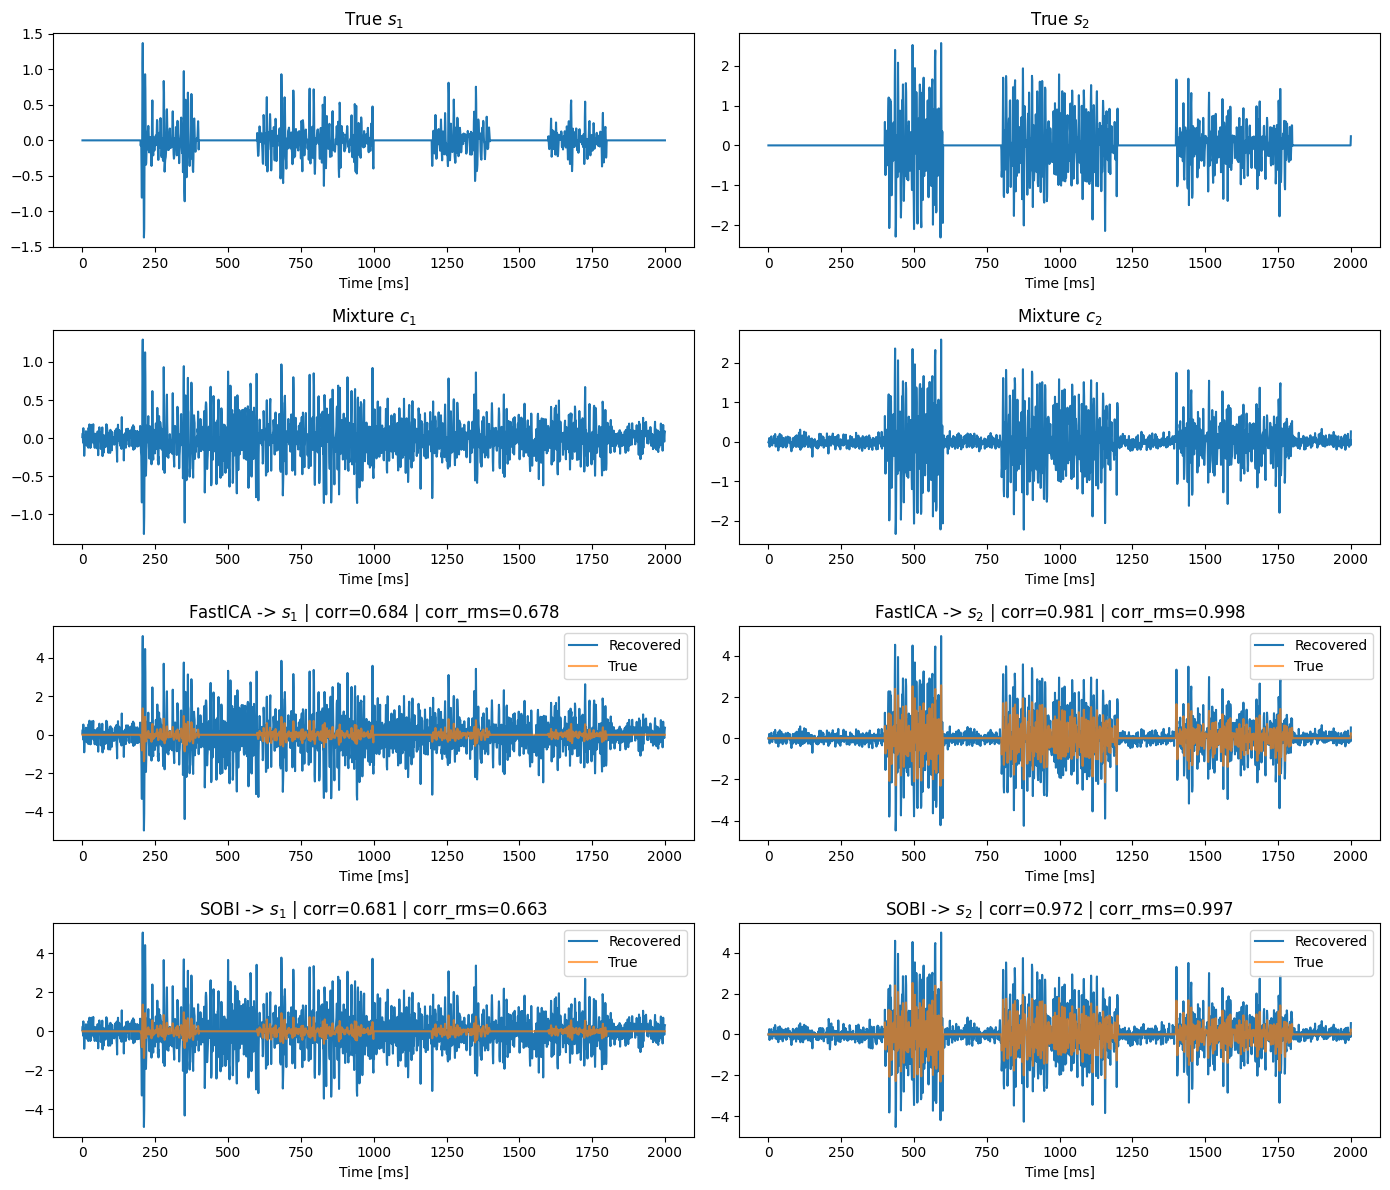
\includegraphics[width=\linewidth,height=12.1cm]{figuras/SOBI/sobi_results_TMR.png}
    }
    \caption{Comparison of the signal separation performed by FastICA and the designed SOBI method in the \textbf{TMR patients dataset}. Both algorithms achieve similar results as non-gaussianity and temporal structure appear to provide similar information about the original sources.}
    \label{fig:sobi_results_tmr}
\end{figure}


To evaluate whether SOBI can be actually favorable for the signals in this dataset, the autocorrelation functions of the original sources were computed. Figure \ref{fig:sobi_tmr_autocorr} shows the normalized autocorrelation of both signals. The results point to the fact that both sources present temporal structure at small lags, but their autocorrelation functions become close to zero and oscillate around as the lag increases. In fact, during the first few lags, both curves follow a very similar pattern. All of this suggests that the temporal information available for SOBI is limited, since the sources in this dataset do not present significantly distinguishable autocorrelation structures.

\begin{figure}[H]
    \centering
    \makebox[\textwidth][c]{%
        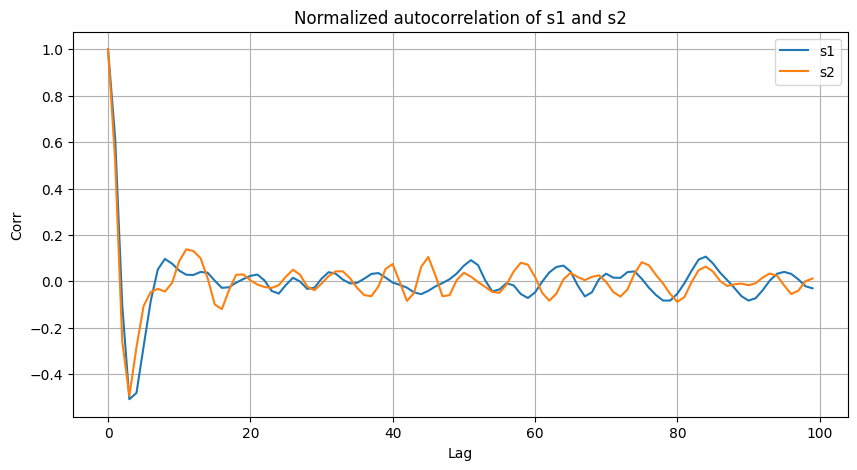
\includegraphics[width=\linewidth, height=7cm]{figuras/SOBI/TMR_norm_autocorr.png}
    }
    \caption{Normalized autocorrolation function for both $s_1$ and $s_2$ in the \textbf{TMR patients dataset}. Both sources have similar autorrelation functions, especially for smaller lags.}
    \label{fig:sobi_tmr_autocorr}
\end{figure}

\subsection{Artificial dataset}

Due to the limited differences observed in the autocorrelation functions of the previous signals, the synthetic dataset introduced in Subsection \ref{subsec:synthetic_dataset} was also considered. As explained previously, this dataset was designed to simulate EMG signals from different muscles under controlled conditions \cite{hamilton-wright_physiologically_2005}. This makes it possible to evaluate SOBI in a scenario where the sources present different temporal autocorrelation structures. Figure \ref{fig:sobi_artificial_autocorr} illustrates the normalized autocorrelation of the selected two sources in this new dataset, which display a significant different behavior overall. 


\begin{figure}[H]
    \centering
    \makebox[\textwidth][c]{%
        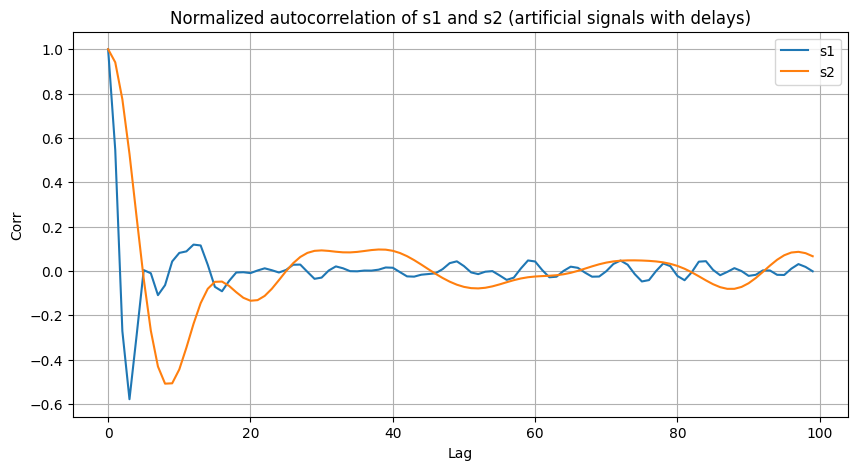
\includegraphics[width=\linewidth,height=6cm]{figuras/SOBI/artificial_norm_autocorr.png}
    }
    \caption{Normalized autocorrolation function for both $s_1$ and $s_2$ in \textbf{the synthetic dataset}. These new sources now present more different autocorrelation functions.}
    \label{fig:sobi_artificial_autocorr}
\end{figure}

However, in practice this does not mean that ICA is outperformed by SOBI in this dataset. Figure \ref{fig:sobi_results_artificial_1} graphically shows that an almost identical separation in the experiment performed with the new synthetic data. Though both algorithms work well under worse conditions ($\sigma=0.1$, $\beta=0.8$ and $\tau=8$ms ), SOBI does not present a significant improvement over ICA. 

\begin{figure}[H]
    \centering
    \makebox[\textwidth][c]{%
        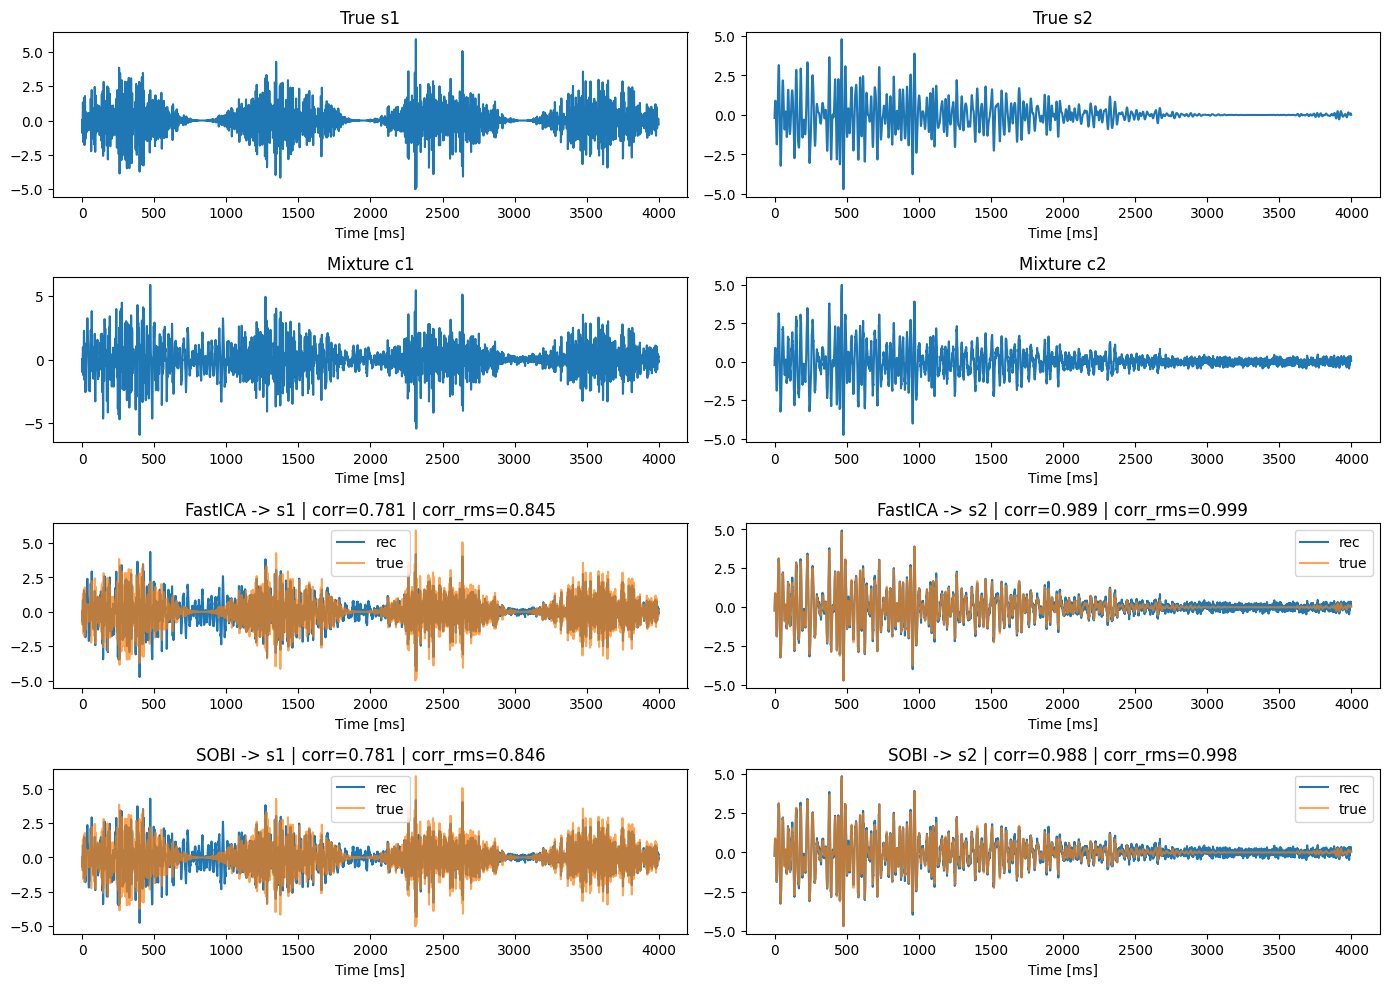
\includegraphics[width=\linewidth]{figuras/SOBI/sobi_results_artificial_1.png}
    }
    \caption{Comparison of ICA and SOBI in the new synthetics data. Parameters were set to $\sigma=0.1$, $\beta=0.8$ and $\tau=\qty{8}{ms}$. Results seem to indicate that the new temporal structure of the signals provide similar information as non-Gaussianity. }
    \label{fig:sobi_results_artificial_1}
\end{figure}



These results suggest that alternating or non-simultaneous EMG activations may
increase the differences in sparsity and amplitude distribution between sources.
As a result, the non-Gaussianity exploited by ICA can provide more
information than the second-order temporal structure exploited by SOBI.

This raises the question: under which conditions would SOBI be preferred over ICA? That would happen when the temporal structure of the sources is significantly more important than their non-Gaussianity. For this reason, Figure \ref{fig:sobi_results_artificial_2}  illustrates the algorithms performance in an artificial scenario in which both EMG sources are simultaneously and share similar envelope, but present different activation frequencies. 


\begin{figure}[H]
    \centering
    \makebox[\textwidth][c]{%
        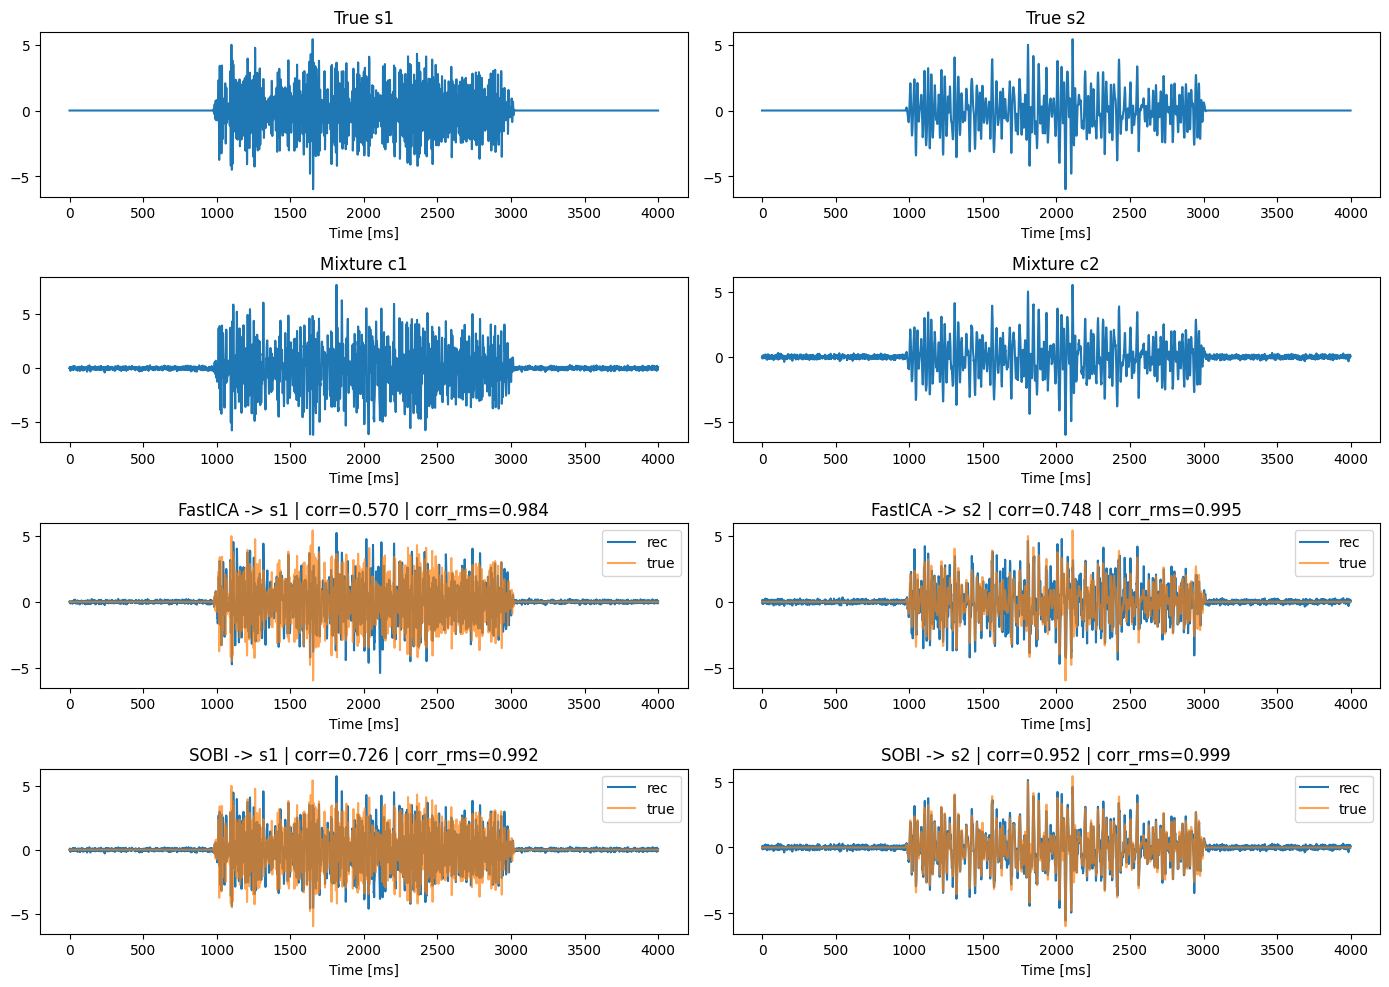
\includegraphics[width=\linewidth]{figuras/SOBI/sobi_results_artificial_2.png}
    }
    \caption{Separation under SOBI favorable artificial scenario. Simultaneous EMG sources present similar envelopes, but have different temporal structures. Parameters were set to $\sigma=0.1$, $\beta=0.8$ and $\tau=\qty{8}{ms}$. In this scenario, SOBI achieves a significant improvement in temporal correlation over ICA, but obtains similar RMS envelope correlations.}
    \label{fig:sobi_results_artificial_2}
\end{figure}



In this case, SOBI shows a clear improvement over ICA in terms of waveform correlation, which indicates better recovery of the temporal structure of the sources. However, even under this favorable scenario for SOBI, both separation algorithms achieve similar RMS envelope correlations. This suggests that, even though SOBI recovers with more detail the temporal waveform, both methods capture the overall activation pattern with similar accuracy. 


\subsection{SOBI experiments conclusion}
\label{subsec:sobi_conclusion}

Overall, although SOBI is a useful blind source separation method, the results
obtained suggest that, for the EMG signals considered in this work,
non-Gaussianity provides more relevant information than second-order
temporal structure. In particular, the autocorrelation functions were often not
different enough to give SOBI a clear advantage over ICA.

Since the main objective of this study is to recover the activation pattern of
the target source and ICA demonstrated better performance for this, the next
step is to improve the ICA algorithm. Therefore, the following chapter
focuses on a modified version of ICA in which additional optimization constraints
are introduced to guide the separation towards the desired source.
